\documentclass[a4paper]{article}
\usepackage[margin=1in]{geometry}%设置边距,符合Word设定
\usepackage{amssymb,amsfonts,amsmath,amsthm}
\usepackage{ctex}
\usepackage{setspace}
\usepackage{lipsum}
\usepackage{graphicx}%插入图片
\usepackage{listings}
\graphicspath{{Figures/}}%文章所用图片在当前目录下的 Figures目录

\usepackage{hyperref} % 对目录生成链接,注:该宏包可能与其他宏包冲突,故放在所有引用的宏包之后
\hypersetup{colorlinks = true,  % 将链接文字带颜色
	bookmarksopen = true, % 展开书签
	bookmarksnumbered = true, % 书签带章节编号
	pdftitle = 数电课设报告, % 标题
	pdfauthor =刘正浩 2019270103005,李仁轩 2019270103011,唐晨烨 2019270103003} % 作者
\bibliographystyle{plain}% 参考文献引用格式
\newcommand{\upcite}[1]{\textsuperscript{\cite{#1}}}

\renewcommand{\contentsname}{\centerline{Contents}} %经过设置word格式后,将目录标题居中


\title{\heiti\zihao{2} 数电课设报告}				%title
\author{\songti 刘正浩 2019270103005,李仁轩 2019270103011,唐晨烨 2019270103003}
\date{\today}


\begin{document}
	\maketitle
	\thispagestyle{empty}

% \begin{abstract}
% 	\lipsum[2]
% \end{abstract}

\tableofcontents
\newpage
	\section{概述}
		本次数电课程设计的要求是:利用HDL设计一个至少支持8条基本MIPS指令(add、sub、and、or、slt、lw、sw、beq)的MCU,
		并利用Vivado\textregistered 工具和Digilent Basys 3 Artix-7 FPGA Board进行MCU的上板验证,
		验证内容为8条基本指令,以及排序算法、DCT算法的二选一实现。\par
	\section{背景及意义}
		在这学期数电课的学习过程中,可以说我们了解了从零开始构建一个完整的CPU的过程。课程的内容包括从晶体管到门电路,
		再到组合电路、时序电路、逻辑块、状态机、FPGA和PLC,以及不同的指令集、处理器架构、I/O设备和存储器等一系列知识。
		有了这些知识,我们就可以以它们为基础来尝试制作一些基本的逻辑电路,最后可以实现一个简单的MCU。
		在设计MCU的过程中也可以检验我们平时的学习情况以及对知识的掌握程度。\par
	\section{目标及完成情况}
		\subsection{目标}
		\begin{enumerate}
			\item 完成MCU中的关键部分之一——ALU的设计与实现。
			\item 选定要实现的MCU的类型,设计结构。
			\item 完成指令集与机器码的设计与互相对应。
			\item 完成MCU的设计。
		\end{enumerate}
		\subsection{完成情况}
			\subsubsection{ALU的设计与实现}
				根据MCU完成必要指令的需要,ALU至少需要支持两个32位数加减、逻辑与或和判断大小的功能。具体的功能和控制信号列表如表\ref{ALU function}。
				\begin{table}[htbp]
					\centering
					\begin{tabular}{c|c}
					\hline
					F(2:0) & Function \\ \hline
					000    & A AND B  \\ \hline
					001    & A OR B   \\ \hline
					010    & A + B    \\ \hline
					011    & reserved \\ \hline
					100    & A AND B' \\ \hline
					101    & A OR B'  \\ \hline
					110    & A - B    \\ \hline
					111    & SLT(比较大小)      \\ \hline
					\end{tabular}
					\caption{ALU功能及对应控制信号}
					\label{ALU function}
				\end{table}

				ALU的结构如图\ref{ALU structure}。
				\begin{figure}[htbp]
					\centering
					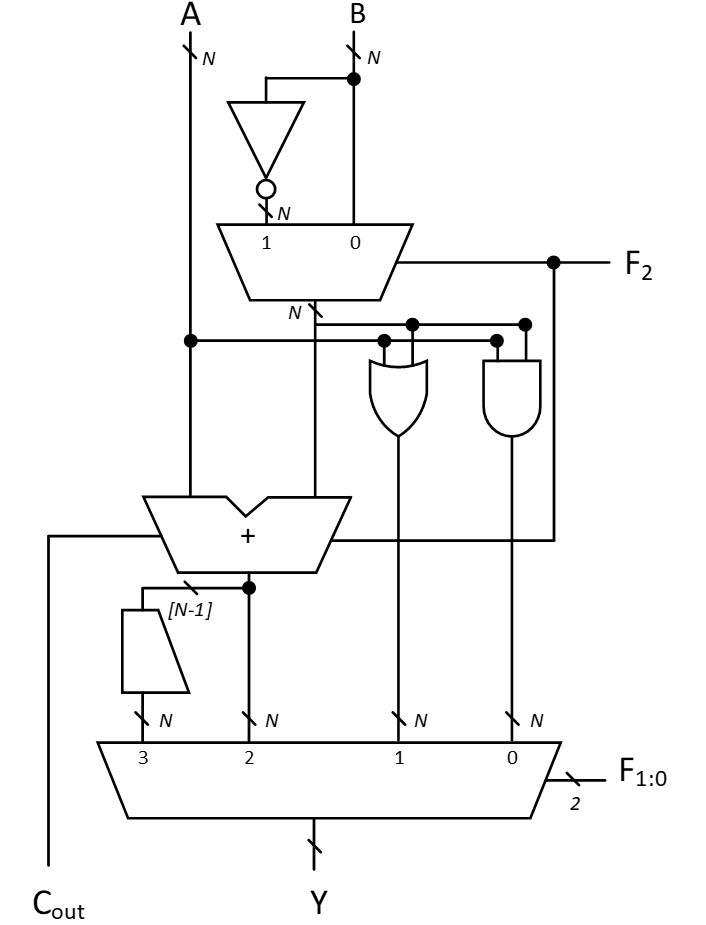
\includegraphics[scale=0.35]{ALU结构.png}
					\caption{ALU结构(图中N=32)}
					\label{ALU structure}
				\end{figure}
				经过测试,ALU的所有功能工作正常。
			\subsubsection{指令集、机器码与MCU的设计与实现}
				由于时间比较紧迫,我们选择了比较简单的单周期MCU制作。具体的结构参考了《数字设计和计算机体系结构》书中所提到的单周期MIPS处理器结构。
				经过测验,我们的处理器实现了八条基本指令,并且可以运行排序算法。具体的设计请见详细设计报告。
	\section{关键创新点及效果}
		\subsection{关于ALU的SLT功能的实现}
			我们规定,当ALU的控制信号为“111”时,ALU进行SLT操作,即比较两个输入的数的大小,如果A<B则输出的结果Y为"0...01",否则输出的32位全为0。
			一种常规的方法是利用A-B的值与0相比较,如果A-B>0则A>B。但我们采用了不同于这种方法的另一种方法。我们分别考察最高位的三个输入,分别是A(31),B(31)和SUM(31)(SUM为A-B的值)。
			构造这三个变量作为输入,Y的最低位作为输出的卡诺图,进而得到一个简单的组合电路。画出的卡诺图如表\ref{SLT logic}。\par
			\begin{table}[htbp]
				\centering
				\begin{tabular}{|l|l|l|l|l|}
					\hline
					AB and SUM & 00 & 01 & 11 & 10 \\ \hline
					    0      & 0  & 0  & 0  & 1  \\ \hline
					    1      & 1  & 0  & 1  & 1  \\ \hline
				\end{tabular}
				\caption{卡诺图}
				\label{SLT logic}
			\end{table}
			得到的化简后的表达式为
			\begin{equation}
				Y_0 =A_{31} \cdot B_{31}' +  A_{31} \cdot SUM_{31} + B_{31}' \cdot SUM_{31}
			\end{equation}
			根据化简后的式子,就可以搭建出相应的逻辑电路。
		\subsection{关于汇编程序}
		对于运算结果的保存,我们采用了无跳转的设计。如果在写入每一位时都判断是否为原最小值所在位置,那么会产生大量跳转指令,浪费很多周期。考虑到此排序问题的特殊性,我们实际上可以对所有位置的先写入最小值,
		而后直接在原最小值位置写入次小值,这样就大大降低了保存结果时的周期消耗(节约了近30个时钟周期)。
	\section{详细设计报告}
		\subsection{硬件架构设计}
			\subsubsection{ALU架构设计}
				在前文中已经提到过ALU的功能列表以及结构设计,这里不在赘述。在ALU中,我们采用了门级描述,单独设计了2:1多路复用器、4:1多路复用器和加法器。
				其中加法器为最简单的行波进位加法器。综合后的ALU结构图如图\ref{ALU after synthesis}。
				
			\subsubsection{MCU架构设计}
				MCU共分为四大部分:控制器、数据通路、RAM和ROM。控制器负责产生所有控制信号,数据通路负责数据和立即数的运算,RAM中存放原式数据和运算后的数据,ROM中存放汇编指令。
				MCU的结构如图\ref{MCU structure}。
				\begin{figure}[htbp]
					\centering
					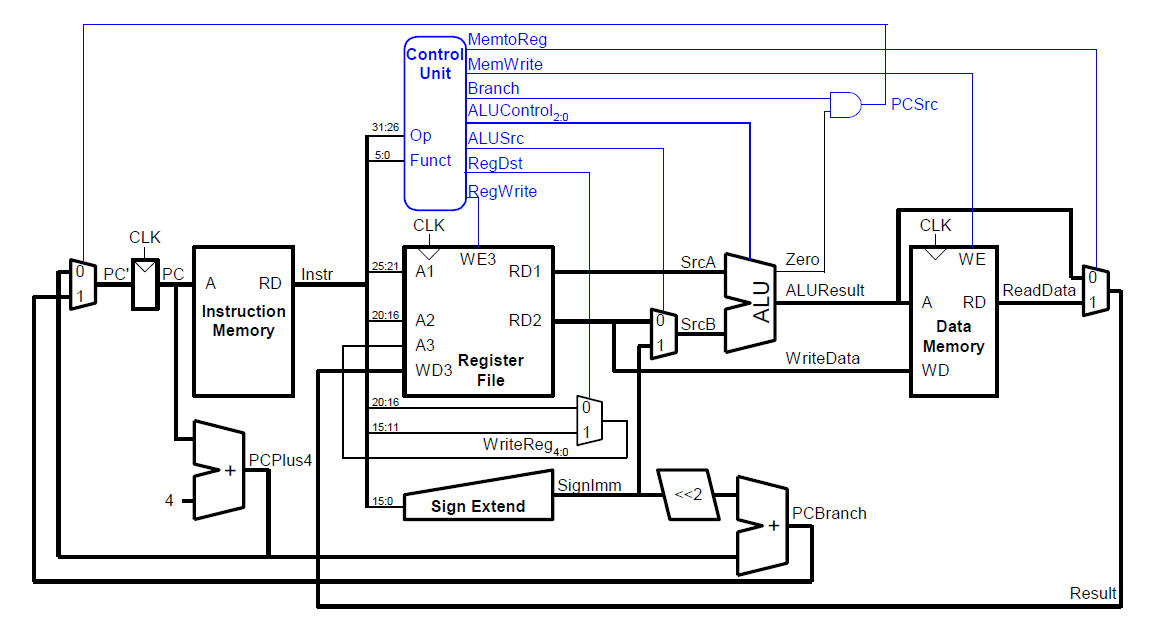
\includegraphics[scale=0.5]{MCU结构.png}
					\caption{MCU结构}
					\label{MCU structure}
				\end{figure}
				其中,Instruction Memory(ROM)和Data Memory(RAM)通过调用IP核“Distributed Memory Generator”来实现,其余部分通过编写HDL文件实现。\par

				Datapath(数据路径)中主要包括寄存器文件、ALU、PC(program counter,程序计数器)以及数据选通器几个成分。\par
				寄存器文件即在MCU中的寄存器。我们按照标准的MIPS寄存器集来设计我们的寄存器文件。寄存器集中共有32个寄存器,从0到31进行编号。
				寄存器文件共有七个端口,分别是CLK(时钟)、A1和A2(两个5位读数据地址输入端)、A3(5位写数据地址输入端)、RD1和RD2(两个32位读数据数据端)
				、WD3(32位写数据数据端)和WE3(数据写使能控制端,高电平为写使能)。\par
				ALU即为上文中介绍的ALU。\par
				PC是一个32位寄存器,通过一个加法器来实现PC+4(指向下一条指令)的功能,还可以通过数据选通器以及符号扩展单元的加入来实现向指定的指令地址跳转的功能。\par

				Controller(控制器)分为主译码器和ALU译码器两个部分。控制器负责将机器码中的opcode字段($Instr_{31:26}$)和funct($Instr_{5:0}$)提取出来进行译码,
				得到用于控制MCU各个部分(寄存器文件、ALU、数据存储器以及各个选通器)的信号。主译码器和ALU译码器的真值表分别如图\ref{main decoder truth tabel}和图\ref{ALU decoder truth table}。\par
				\begin{figure}[htbp]
					\centering
					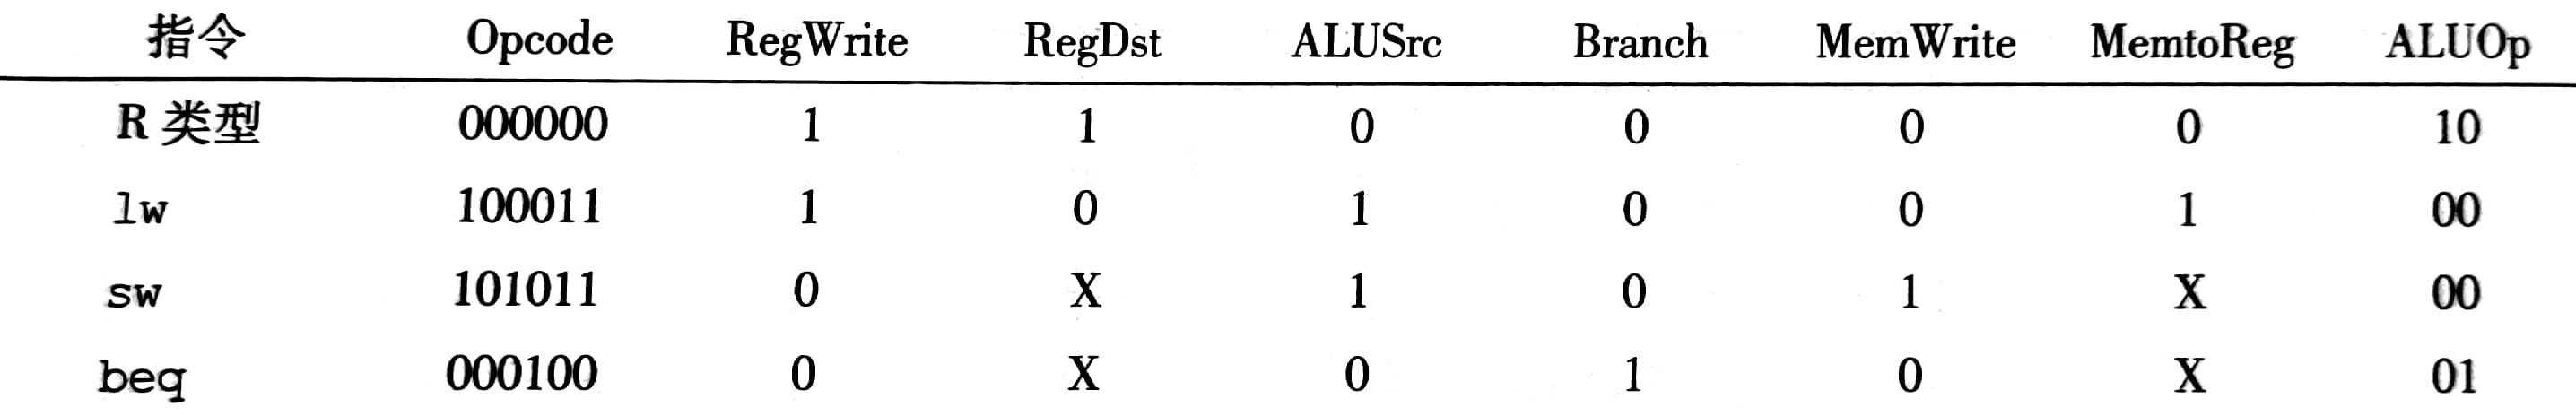
\includegraphics[scale=0.15]{主译码器真值表.jpg}
					\caption{主译码器真值表}
					\label{main decoder truth tabel}
				\end{figure}

				\begin{figure}[htbp]
					\centering
					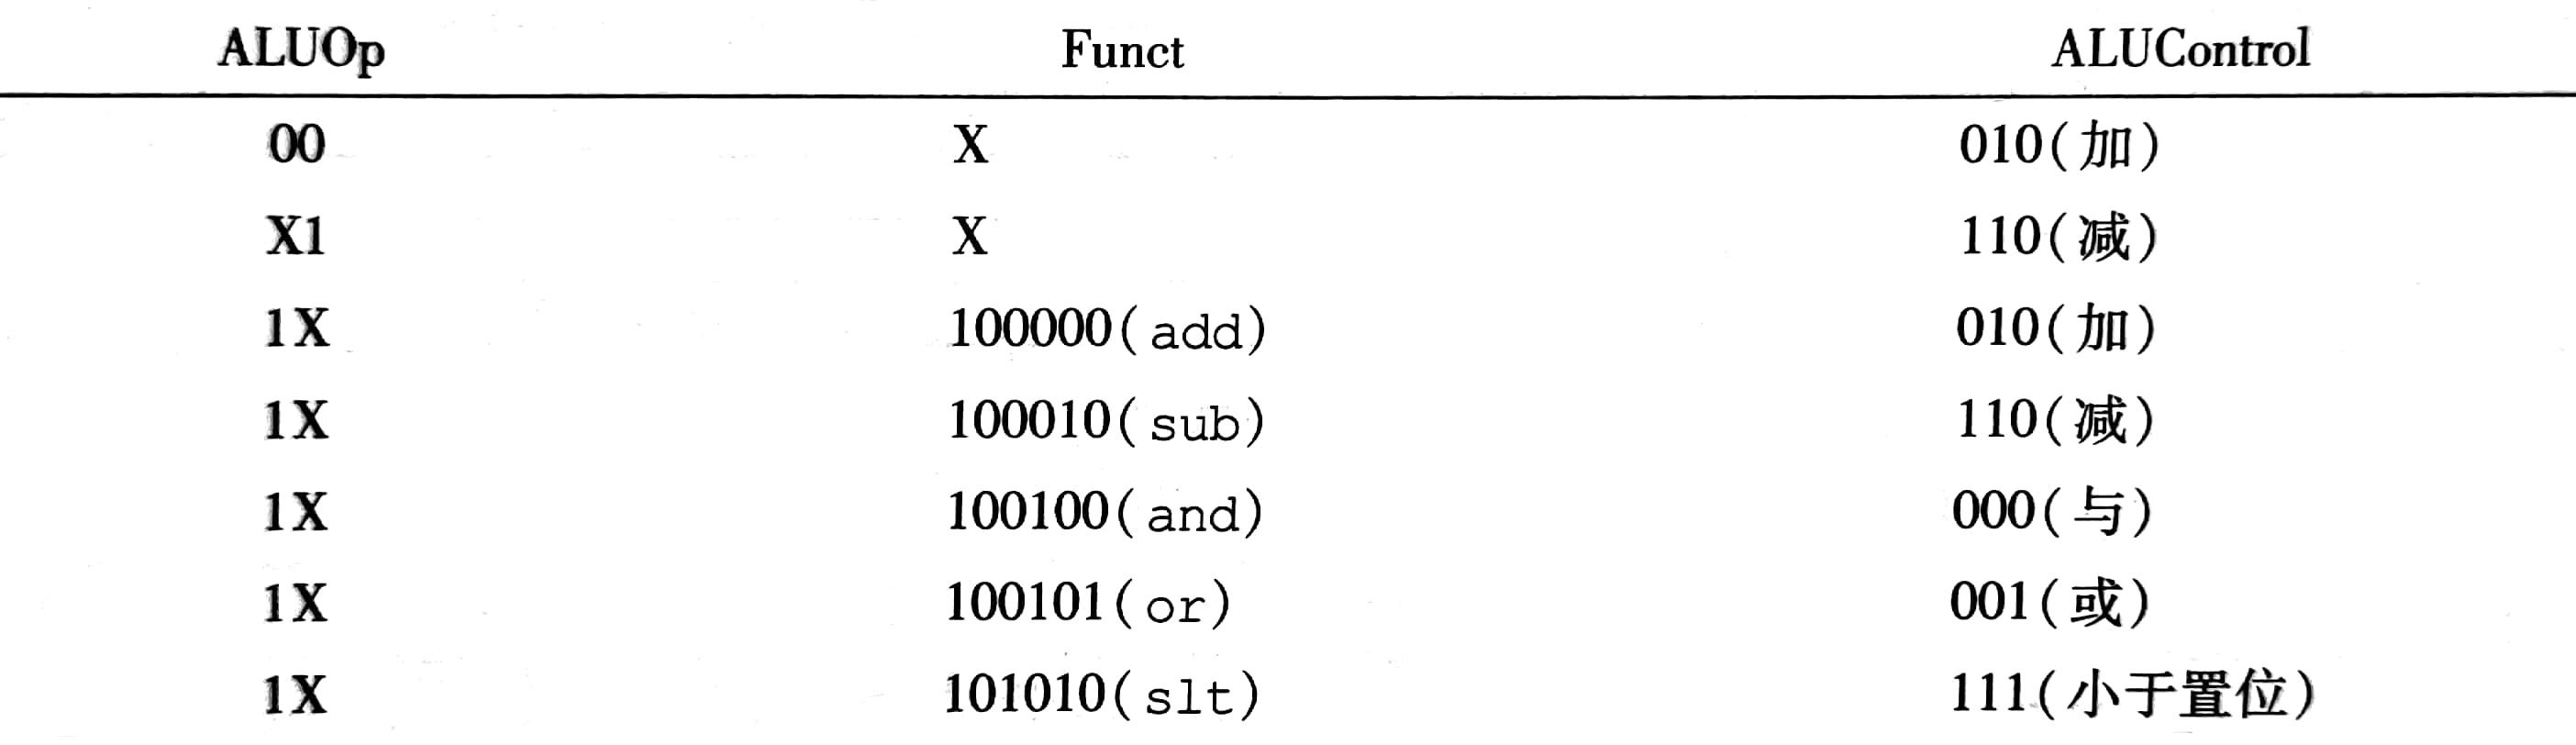
\includegraphics[scale=0.15]{ALU译码器真值表.jpg}
					\caption{ALU译码器真值表}
					\label{ALU decoder truth table}
				\end{figure}

				综合后的MCU结构如图\ref{MCU after synthesis}。资源消耗情况和时序分析结果如图\ref{usage and timing analysis}。其中ILA(Integrated Logic Analyzer,集成逻辑分析仪)
				是为了检测MCU内部信号情况而调用的IP核,不计算在MCU的消耗中。这样,MCU就总共消耗了836个LUT(Look up table,查找表)和745个FF(Flip flop,触发器)。
				\begin{figure}[htbp]
					\centering
					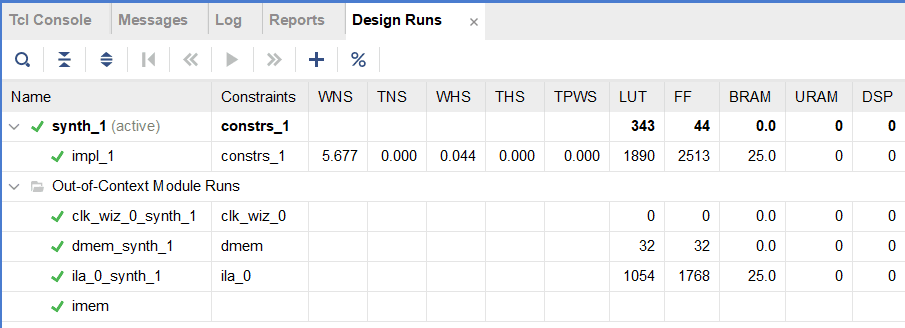
\includegraphics[scale=0.45]{资源消耗和时序分析.png}
					\caption{资源消耗和时序分析结果}
					\label{usage and timing analysis}
				\end{figure}
				\begin{figure}[htbp]
					\centering
					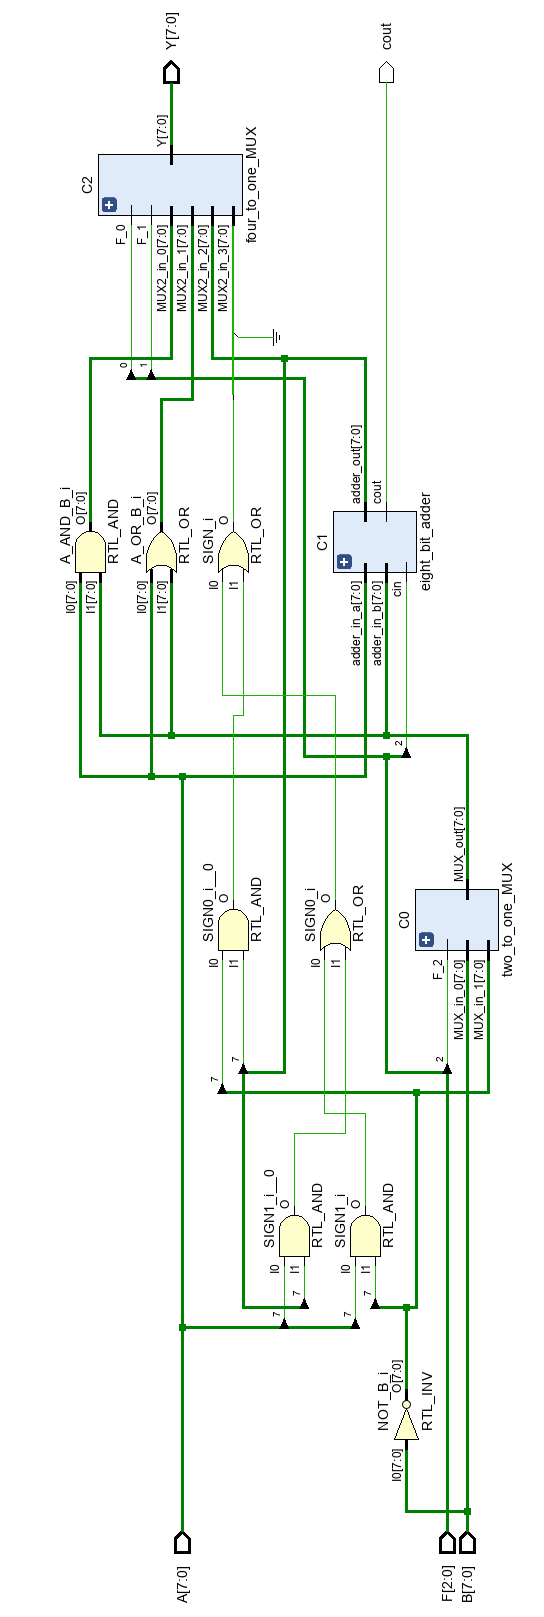
\includegraphics[scale=0.55]{综合后的ALU.png}
					\caption{综合后的ALU}
					\label{ALU after synthesis}
				\end{figure}
				\begin{figure}[htbp]
					\centering
					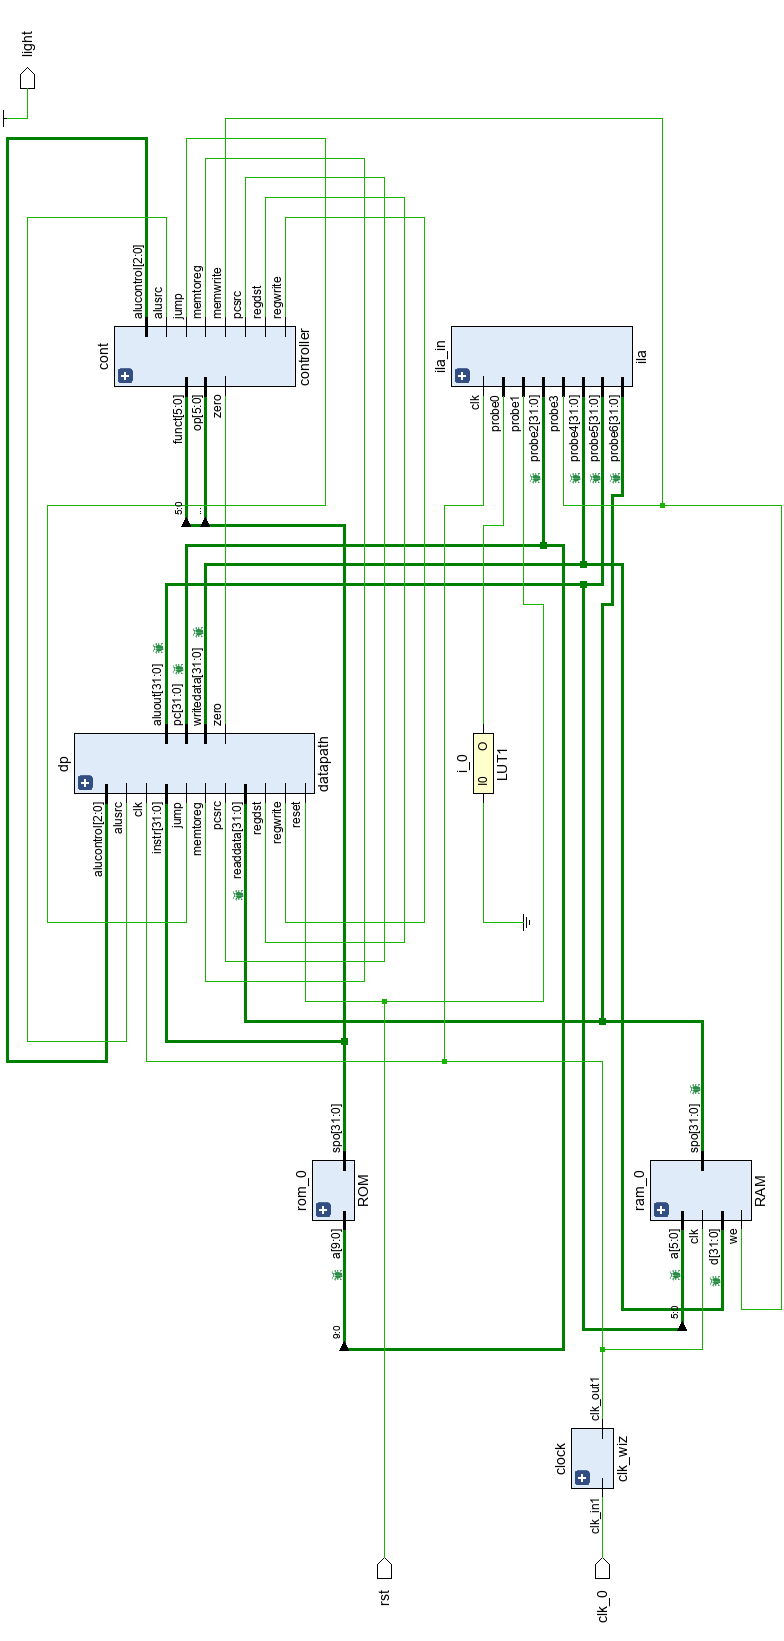
\includegraphics[scale=0.5]{综合后的MCU.png}
					\caption{综合后的MCU}
					\label{MCU after synthesis}
				\end{figure}
				\newpage

		\subsection{软件设计}
		优化方法:由于寄存器有限,考虑到问题的特殊性,故分两次读入数据。采用“打擂台”方式取得最小值、次小值和最小值位置:
		即每次将输入值与最小值和次小值分别比较并更新,如果小于最小值则更新最小值、次小值、最小值位置,如果只小于次小值则只更新次小值。采用无跳转设计来减少写入时花费的周期数。
		下附完整的汇编代码和机器码。
			\subsubsection{汇编代码}
			\lstset{language=VHDL}
			\begin{lstlisting}
		add $t0,$0,$0 #初始化
		add $t1,$0,$0
		add $t2,$0,$0
		add $t3,$0,$0
		lw $s0,0x0000($0) #读入第一批数据
		lw $s1,0x0001($0)
		lw $s2,0x0002($0)
		lw $s3,0x0003($0)
		lw $s4,0x0004($0)
		lw $s5,0x0005($0)
		lw $s6,0x0006($0)
		lw $s7,0x0007($0)
		slt $t2,$s0,$0 #取绝对值
		beq $t2,$0,a0
		sub $s0,$0,$s0
	a0: slt $t2,$s1,$0
		beq $t2,$0,a1
		sub $s1,$0,$s1
	a1: slt $t2,$s2,$0
		beq $t2,$0,a2
		sub $s2,$0,$s2
	a2: slt $t2,$s3,$0
		beq $t2,$0,a3
		sub $s3,$0,$s3
	a3: slt $t2,$s4,$0
		beq $t2,$0,a4
		sub $s4,$0,$s4
	a4: slt $t2,$s5,$0
		beq $t2,$0,a5
		sub $s5,$0,$s5
	a5: slt $t2,$s6,$0
		beq $t2,$0,a6
		sub $s6,$0,$s6
	a6: slt $t2,$s7,$0
		beq $t2,$0,a7
		sub $s7,$0,$s7
	a7: add $t0,$s0,$0 #初始化最小值、次小值、最小值位置
		slt $t2,$s1,$t0
		beq $t2,$0,b1
		add $t1,$t0,$0
		add $t0,$s1,$0
		addi $t3,$0,0x0001
		beq $0,$0,c1
	b1: add $t1,$s1,$0
	c1: slt $t2,$s2,$t1 #打擂台
		beq $t2,$0,c2
		slt $t2,$s2,$t0
		beq $t2,$0,b2
		add $t1,$t0,$0
		add $t0,$s2,$0
		addi $t3,$0,0x0002
		beq $0,$0,c2
	b2: add $t1,$s2,$0
	c2: slt $t2,$s3,$t1
		beq $t2,$0,c3
		slt $t2,$s3,$t0
		beq $t2,$0,b3
		add $t1,$t0,$0
		add $t0,$s3,$0
		addi $t3,$0,0x0003
		beq $0,$0,c3
	b3: add $t1,$s3,$0
	c3: slt $t2,$s4,$t1
		beq $t2,$0,c4
		slt $t2,$s4,$t0
		beq $t2,$0,b4
		add $t1,$t0,$0
		add $t0,$s4,$0
		addi $t3,$0,0x0004
		beq $0,$0,c4
	b4: add $t1,$s4,$0
	c4: slt $t2,$s5,$t1
		beq $t2,$0,c5
		slt $t2,$s5,$t0
		beq $t2,$0,b5
		add $t1,$t0,$0
		add $t0,$s5,$0
		addi $t3,$0,0x0005
		beq $0,$0,c5
	b5: add $t1,$s5,$0
	c5: slt $t2,$s6,$t1
		beq $t2,$0,c6
		slt $t2,$s6,$t0
		beq $t2,$0,b6
		add $t1,$t0,$0
		add $t0,$s6,$0
		addi $t3,$0,0x0006
		beq $0,$0,c6
	b6: add $t1,$s6,$0
	c6: slt $t2,$s7,$t1
		beq $t2,$0,c7
		slt $t2,$s7,$t0
		beq $t2,$0,b7
		add $t1,$t0,$0
		add $t0,$s7,$0
		addi $t3,$0,0x0007
		beq $0,$0,c7
	b7: add $t1,$s7,$0
	c7: lw $s0,0x0008($0) #读入第二批数据
		lw $s1,0x0009($0)
		lw $s2,0x000A($0)
		lw $s3,0x000B($0)
		lw $s4,0x000C($0)
		lw $s5,0x000D($0)
		lw $s6,0x000E($0)
		lw $s7,0x000F($0)
		slt $t2,$s0,$0 #取绝对值
		beq $t2,$0,d0
		sub $s0,$0,$s0
	d0: slt $t2,$s1,$0
		beq $t2,$0,d1
		sub $s1,$0,$s1
	d1: slt $t2,$s2,$0
		beq $t2,$0,d2
		sub $s2,$0,$s2
	d2: slt $t2,$s3,$0
		beq $t2,$0,d3
		sub $s3,$0,$s3
	d3: slt $t2,$s4,$0
		beq $t2,$0,d4
		sub $s4,$0,$s4
	d4: slt $t2,$s5,$0
		beq $t2,$0,d5
		sub $s5,$0,$s5
	d5: slt $t2,$s6,$0
		beq $t2,$0,d6
		sub $s6,$0,$s6
	d6: slt $t2,$s7,$0
		beq $t2,$0,d7
		sub $s7,$0,$s7
	d7: slt $t2,$s0,$t1 #打擂台
		beq $t2,$0,f0
		slt $t2,$s0,$t0
		beq $t2,$0,e0
		add $t1,$t0,$0
		add $t0,$s0,$0
		addi $t3,$0,0x0008
		beq $0,$0,f0
	e0: add $t1,$s0,$0
	f0: slt $t2,$s1,$t1
		beq $t2,$0,f1
		slt $t2,$s1,$t0
		beq $t2,$0,e1
		add $t1,$t0,$0
		add $t0,$s1,$0
		addi $t3,$0,0x0009
		beq $0,$0,f1
	e1: add $t1,$s1,$0
	f1: slt $t2,$s2,$t1
		beq $t2,$0,f2
		slt $t2,$s2,$t0
		beq $t2,$0,e2
		add $t1,$t0,$0
		add $t0,$s2,$0
		addi $t3,$0,0x000A
		beq $0,$0,f2
	e2: add $t1,$s2,$0
	f2: slt $t2,$s3,$t1
		beq $t2,$0,f3
		slt $t2,$s3,$t0
		beq $t2,$0,e3
		add $t1,$t0,$0
		add $t0,$s3,$0
		addi $t3,$0,0x000B
		beq $0,$0,f3
	e3: add $t1,$s3,$0
	f3: slt $t2,$s4,$t1
		beq $t2,$0,f4
		slt $t2,$s4,$t0
		beq $t2,$0,e4
		add $t1,$t0,$0
		add $t0,$s4,$0
		addi $t3,$0,0x000C
		beq $0,$0,f4
	e4: add $t1,$s4,$0
	f4: slt $t2,$s5,$t1
		beq $t2,$0,f5
		slt $t2,$s5,$t0
		beq $t2,$0,e5
		add $t1,$t0,$0
		add $t0,$s5,$0
		addi $t3,$0,0x000D
		beq $0,$0,f5
	e5: add $t1,$s5,$0
	f5: slt $t2,$s6,$t1
		beq $t2,$0,f6
		slt $t2,$s6,$t0
		beq $t2,$0,e6
		add $t1,$t0,$0
		add $t0,$s6,$0
		addi $t3,$0,0x000E
		beq $0,$0,f6
	e6: add $t1,$s6,$0
	f6: slt $t2,$s7,$t1
		beq $t2,$0,f7
		slt $t2,$s7,$t0
		beq $t2,$0,e7
		add $t1,$t0,$0
		add $t0,$s7,$0
		addi $t3,$0,0x000F
		beq $0,$0,f7
	e7: add $t1,$s7,$0
	f7: sw $t0,0x0010($0) #写入最小值
		sw $t0,0x0011($0)
		sw $t0,0x0012($0)
		sw $t0,0x0013($0)
		sw $t0,0x0014($0)
		sw $t0,0x0015($0)
		sw $t0,0x0016($0)
		sw $t0,0x0017($0)
		sw $t0,0x0018($0)
		sw $t0,0x0019($0)
		sw $t0,0x001A($0)
		sw $t0,0x001B($0)
		sw $t0,0x001C($0)
		sw $t0,0x001D($0)
		sw $t0,0x001E($0)
		sw $t0,0x001F($0)
		sw $t1,0x0010($t3) #写入次小值
			\end{lstlisting}

			\subsubsection{机器码}
			\lstset{language=VHDL}
			\begin{lstlisting}
	memory_initialization_radix = 16;
	memory_initialization_vector = 
				00004020,
				00004820,
				00005020,
				00005820,
				8c100000,
				8c110001,
				8c120002,
				8c130003,
				8c140004,
				8c150005,
				8c160006,
				8c170007,
				0200502a,
				11400001,
				00108022,
				0220502a,
				11400001,
				00118822,
				0240502a,
				11400001,
				00129022,
				0260502a,
				11400001,
				00139822,
				0280502a,
				11400001,
				0014a022,
				02a0502a,
				11400001,
				0015a822,
				02c0502a,
				11400001,
				0016b022,
				02e0502a,
				11400001,
				0017b822,
				02004020,
				0228502a,
				11400004,
				01004820,
				02204020,
				200b0001,
				10000001,
				02204820,
				0249502a,
				11400007,
				0248502a,
				11400004,
				01004820,
				02404020,
				200b0002,
				10000001,
				02404820,
				0269502a,
				11400007,
				0268502a,
				11400004,
				01004820,
				02604020,
				200b0003,
				10000001,
				02604820,
				0289502a,
				11400007,
				0288502a,
				11400004,
				01004820,
				02804020,
				200b0004,
				10000001,
				02804820,
				02a9502a,
				11400007,
				02a8502a,
				11400004,
				01004820,
				02a04020,
				200b0005,
				10000001,
				02a04820,
				02c9502a,
				11400007,
				02c8502a,
				11400004,
				01004820,
				02c04020,
				200b0006,
				10000001,
				02c04820,
				02e9502a,
				11400007,
				02e8502a,
				11400004,
				01004820,
				02e04020,
				200b0007,
				10000001,
				02e04820,
				8c100008,
				8c110009,
				8c12000a,
				8c13000b,
				8c14000c,
				8c15000d,
				8c16000e,
				8c17000f,
				0200502a,
				11400001,
				00108022,
				0220502a,
				11400001,
				00118822,
				0240502a,
				11400001,
				00129022,
				0260502a,
				11400001,
				00139822,
				0280502a,
				11400001,
				0014a022,
				02a0502a,
				11400001,
				0015a822,
				02c0502a,
				11400001,
				0016b022,
				02e0502a,
				11400001,
				0017b822,
				0209502a,
				11400007,
				0208502a,
				11400004,
				01004820,
				02004020,
				200b0008,
				10000001,
				02004820,
				0229502a,
				11400007,
				0228502a,
				11400004,
				01004820,
				02204020,
				200b0009,
				10000001,
				02204820,
				0249502a,
				11400007,
				0248502a,
				11400004,
				01004820,
				02404020,
				200b000a,
				10000001,
				02404820,
				0269502a,
				11400007,
				0268502a,
				11400004,
				01004820,
				02604020,
				200b000b,
				10000001,
				02604820,
				0289502a,
				11400007,
				0288502a,
				11400004,
				01004820,
				02804020,
				200b000c,
				10000001,
				02804820,
				02a9502a,
				11400007,
				02a8502a,
				11400004,
				01004820,
				02a04020,
				200b000d,
				10000001,
				02a04820,
				02c9502a,
				11400007,
				02c8502a,
				11400004,
				01004820,
				02c04020,
				200b000e,
				10000001,
				02c04820,
				02e9502a,
				11400007,
				02e8502a,
				11400004,
				01004820,
				02e04020,
				200b000f,
				10000001,
				02e04820,
				ac080010,
				ac080011,
				ac080012,
				ac080013,
				ac080014,
				ac080015,
				ac080016,
				ac080017,
				ac080018,
				ac080019,
				ac08001a,
				ac08001b,
				ac08001c,
				ac08001d,
				ac08001e,
				ac08001f,
				ad690010;
				
			\end{lstlisting}
\newpage
	\section{测试报告}
		经过测试,我们的MCU可以运行所有指令,并能够完成排序算法。由于时间紧迫,我们没有对最终的验收成果进行截图。图\ref{ila}为一次中途验收的效果截图。
		图中的存入顺序和数据都是正确的。
		\begin{figure}[htbp]
			\centering
			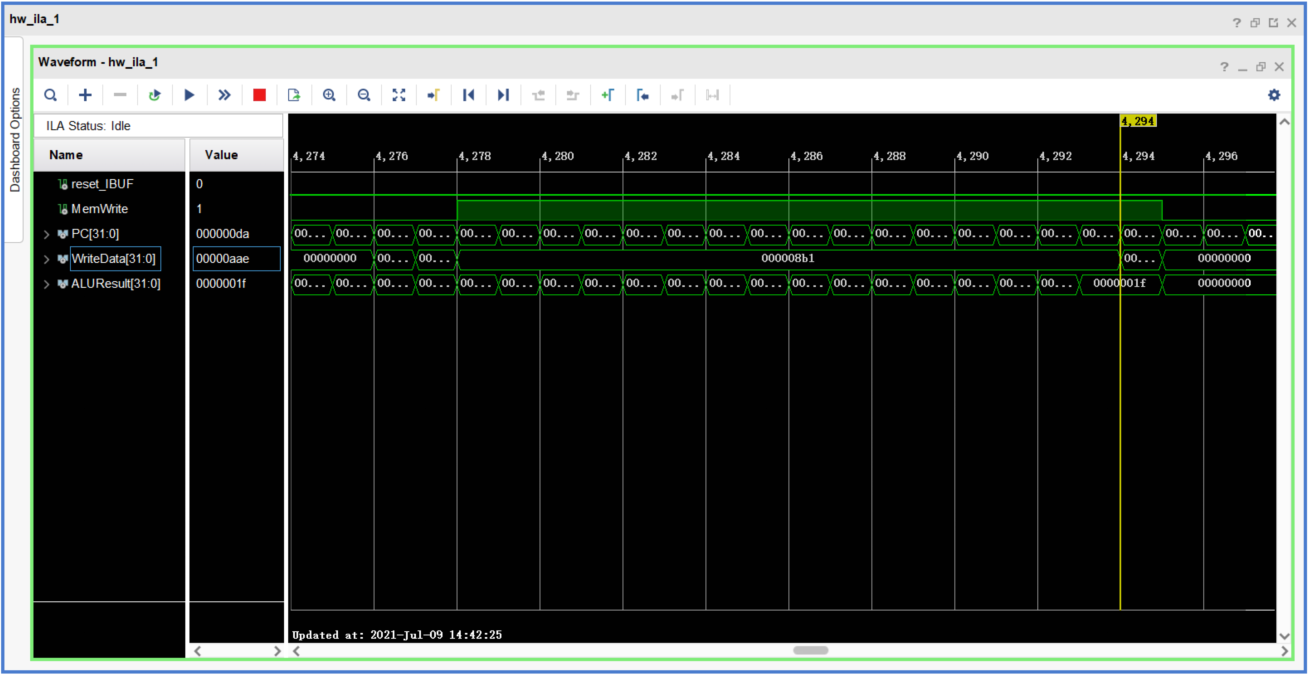
\includegraphics[scale=0.4]{ila.png}
			\caption{中途验证的结果}
			\label{ila}
		\end{figure}

	\section{总结和展望}
		我们这次的课程设计总的来说是成功的。我们从零开始实现了一个完整的MCU,自己完成了算法的设计和汇编语言的书写,受益匪浅。\par
		关于硬件的展望与思索:在设计过程中我们依然走了很多弯路,比如有些地方可以用行为级描述来书写结果却用了门级描述;没有在开始设计前构思好MCU的具体结构,导致中途返工多次,等等。
		这也提示我们今后在进行设计时要多动脑,同时做好规划和总结。\par
		关于算法的展望和思索:如果测试数据的排列顺序为从大到小,则使用当前的算法进行排序时将会消耗较大的时间,浪费很多时钟周期。后续可以通过改进算法来提升运行效率。
\end{document}